\documentclass{article} 
\usepackage{polyglossia} 
\usepackage{amsmath}
\usepackage{fontspec} 
\usepackage{lipsum} 
\usepackage[margin=1in]{geometry}
\usepackage{graphicx} 
\usepackage[figurename=Εικόνα]{caption} 
\usepackage{subcaption}
\usepackage{hyperref} 
\usepackage{listing}
\hypersetup{% 
    colorlinks=true, linkcolor=blue, filecolor=magenta,      
    urlcolor=cyan, 
    pdfinfo = {%
        Title = Αναφορά 3ης Εργασίας ΨΕΕ
        Author = {Χρήστος Μάριος Περδίκης},
        Producer = XeLaTeX,
    } 
}

\renewcommand{\figureautorefname}{Εικόνα}
\setmainfont{Nimbus Roman}

\title{Ψηφιακή Επεξεργασία Εικόνας \\ Image Segmentation}
\date{Εαρινό Εξάμηνο 2024-2025}
\author{Χρήστος-Μάριος Περδίκης 10075 cperdikis@ece.auth.gr}

\begin{document}
\maketitle
Σε αυτήν την εργασία υλοποιείται σε python η αναπαράσταση εικόνων σε γράφους και image
segmentation με τις μεθόδους spectral clustering και normalized cuts.


\section{Συνάρτηση img\_to\_graph()}
Η συνάρτηση img\_to\_graph() βρίσκεται στο αρχείο img\_to\_graph.py. Η είσοδός της
είναι το array της εικόνας εισόδου του προγράμματος. Για να απλουστευτούν οι πράξεις, 
το array της εικόνας 
ανασχηματίζεται έτσι ώστε κάθε γραμμή να αντιστοιχεί σε ένα pixel με C κανάλια. 
Για τον υπολογισμό των ευκλείδιων αποστάσεων 
μεταξύ των pixel της εικόνας χρησιμοποιείται η συνάρτηση scipy.spatial.distance.cdist()
για λόγους αποδοτικότητας. Έπειτα υπολογίζεται το affinity matrix:

\begin{equation}
    \text{affinity\_mat} = \frac{1}{e^{distances}}
\end{equation}
όπου $distances$ το array που περιέχει τις ευκλείδιες αποστάσεις κάθε ζεύγους
pixel στην εικόνα. Τέλος στον πίνακα affinity matrix τοποθετούνται άσσοι στην
διαγώνιό του, για να είναι σίγουρο ότι το ζεύγος ενός pixel με τον εαυτό του
είναι ακριβώς 1 και επιστρέφεται ο πίνακας affinity matrix.

\section{Συνάρτηση spectral\_clustering()}
Η συνάρτηση spectral\_clustering() βρίσκεται στο αρχείο spectral\_clustering().
Η είσοδος της συνάρτησης είναι ένα affinity matrix που περιγράφει τον γράφο μιας
εικόνας και ο ακέραιος k που θα καθορίσει σε πόσα clusters θα χωρίσουμε την εικόνα.
Κατασκευάζεται το degree matrix από το affinity matrix:

\begin{equation}
    D(i, i) = \sum_j W(i, j)
\end{equation}
Έπειτα υπολογίζεται ο Λαπλασιανός πίνακας:

\begin{equation}
    L = D - W
\end{equation}
Βρίσκονται οι ιδιοτιμές και τα ιδιοδιανύσματα του Λαπλασιανού πίνακα. 
\begin{equation}
    Lx = \lambda x
\end{equation}
Η συνάρτηση scipy.sparse.linalg.eigs() καλείται με ορίσματα k=$k$ και 
which='SM', έτσι ώστε η συνάρτηση να επι\-στρέψει τις $k$ μικρότερες σε μέτρο
ιδιοτιμές και τα αντίστοιχα ιδιοδιανύ\-σματα. Ο πίνακας $U$
έχει στήλες τα ιδιοδιανύ\-σματα του Λαπλασιανού πίνακα $L$. Οι γραμμές του
$U$ ομαδοποιούνται με τη μέθοδο k-means clustering με τον τρόπο που περιγράφεται 
στην εκφώνηση της εργασίας. Η συνάρτηση sklearn.cluster.KMeans()
δεν υποστηρίζει φανταστικούς αριθμούς, οπότε ο πίνακας $U$ δημιουργείται με
το πραγματικό μόνο μέρος των ιδιοδιανυσμάτων. Το αποτέλεσμα είναι ένα array με ετικέτες που 
δείχνουν σε ποιό cluster ανήκουν οι κορυφές του γράφου (δηλαδή κάθε pixel της
εικόνας) και είναι η έξοδος της συνάρτησης spectral\_clustering().

\section{Εφαρμογές}
\subsection{demo1} 
Στο demo 1 γίνεται η επίδειξη της συνάρτησης spectral\_clustering(). Ο 
προ-κατασκευασμένος affinity πίνακας d1a φορτώνεται από το αρχείο dip\_hw\_3.mat. 
Έπειτα καλείται η συνάρτηση spectral\_clustering() με είσοδο d1a για τιμές $k = 2,3,4$.
Τέλος γίνεται μονοδιάστατη οπτικοποίηση των αποτελεσμάτων στην οποία φαίνεται 
σε ποιό cluster ανήκει κάθε κόμβος του γράφου. 
Βλέξουμε στην~\autoref{figure1} ότι οι 11 κόμβοι του γράφου που μας δόθηκε
χωρίζονται σε 2, 3 και 4 clusters, ανάλογα με την τιμή του $k$.

\begin{figure}
    \centering
    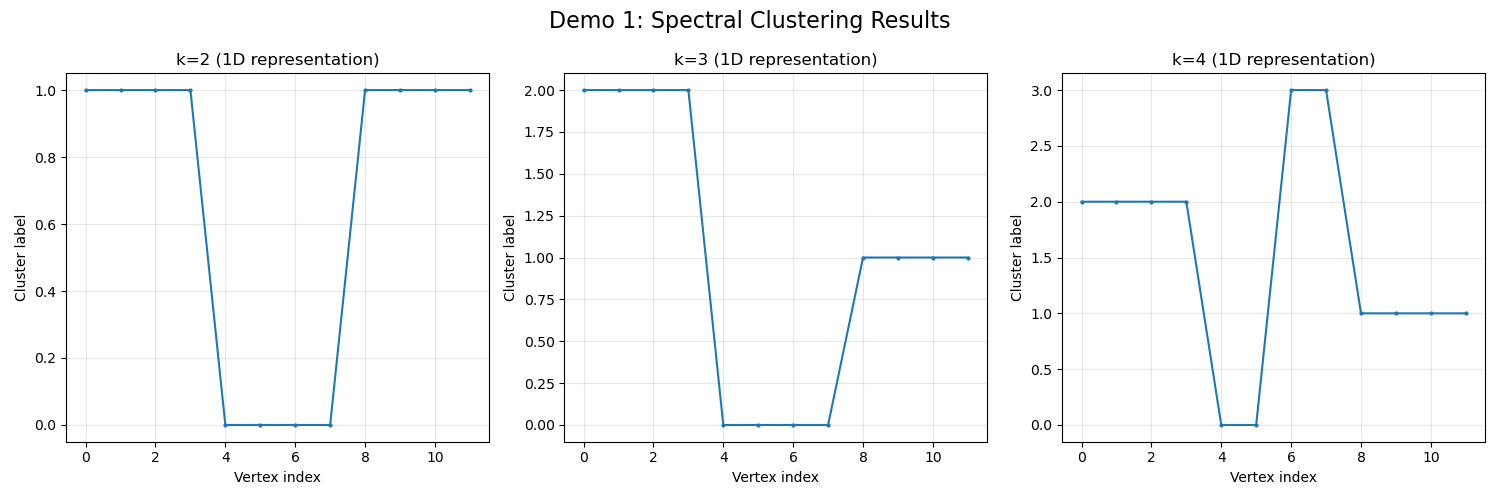
\includegraphics[width=\linewidth]{Figure_1.png}
    \caption{Αποτελέσματα spectral clustering σε έτοιμο affinity matrix}\label{figure1}
\end{figure}


\subsection{demo2}
Στο demo 2 γίνεται η επίδειξη και της συνάρτησης img\_to\_graph() μαζί με τη 
spectral\_clustering(). Οι εικόνες d2a και d2b φορτώνονται από το αρχείο 
dip\_hw\_3.mat. Γίνονται έλεγχοι αν οι εικόνες εισόδου πληρούν τις προϋποθέσεις 
της img\_to\_graph(), δηλαδή αν είναι έγχρωμες και αν οι τιμές των pixel κυμαίνονται 
στο διάστημα $[0,1]$. Για κάθε μία από τις δύο εικόνες υπολογίζεται πρώτα το
affinity matrix με τη χρήση της img\_to\_graph() και αυτό είναι η είσοδος
της spectral\_clustering(). Για κάθε μία από τις δύο εικόνες η συνάρτηση 
spectral\_clustering() τρέχει για τιμές $k = 2,3,4$, συνολικά 6 φορές. Για την
οπτικοποίηση, κάθε cluster από pixels της αρχικής εικόνας έχει διαφορετικό χρώμα. Βλέπουμε 
στην~\autoref{figure2} ότι στην πρώτη εικόνα που μας δόθηκε χωρίζονται σωστά 
οι στήλες χρώματος για $k=2,3$. Για $k=4$ όμως βλέπουμε δύο μικρά κουτάκια 
μέσα στην κόκκινη στήλη, υπάρχει ένα τέταρτο cluster σε μια περιοχή που
στην αρχική εικόνα δεν αλλάζει το χρώμα και δεν έχει λόγο να μην ανήκει στο 
ίδιο cluster. Στη κάτω εικόνα βλέπουμε ότι για $k=2$ στο ένα cluster ανήκουν
τα πολύ άσπρα pixels (οι γωνίες της εικόνας και σημεία από τα γάντια του Mario)
και όλα τα υπόλοιπα pixels στο άλλο cluster. Για $k=3$, στο νέο cluster 
ομαδοποιούνται pixel με κόκκινο ή καφετί χρώμα (τα ρούχα του Mario κάτω από
τη σαλοπέτα, τα παπούτσια του, το καπέλο του, οι φαβορίτες του). Για $k=4$ 
όμως πάλι δεν λαμβάνουμε καμιά νέα πληροφορία για την εικόνα, στο νέο 
cluster ανήκουν pixel από το καπέλο του Mario που στην αρχική εικόνα
έχουν πολύ παρόμοιο χρώμα με το υπόλοιπο καπέλο που ανήκει σε άλλο
cluster.

\begin{figure}
    \centering
    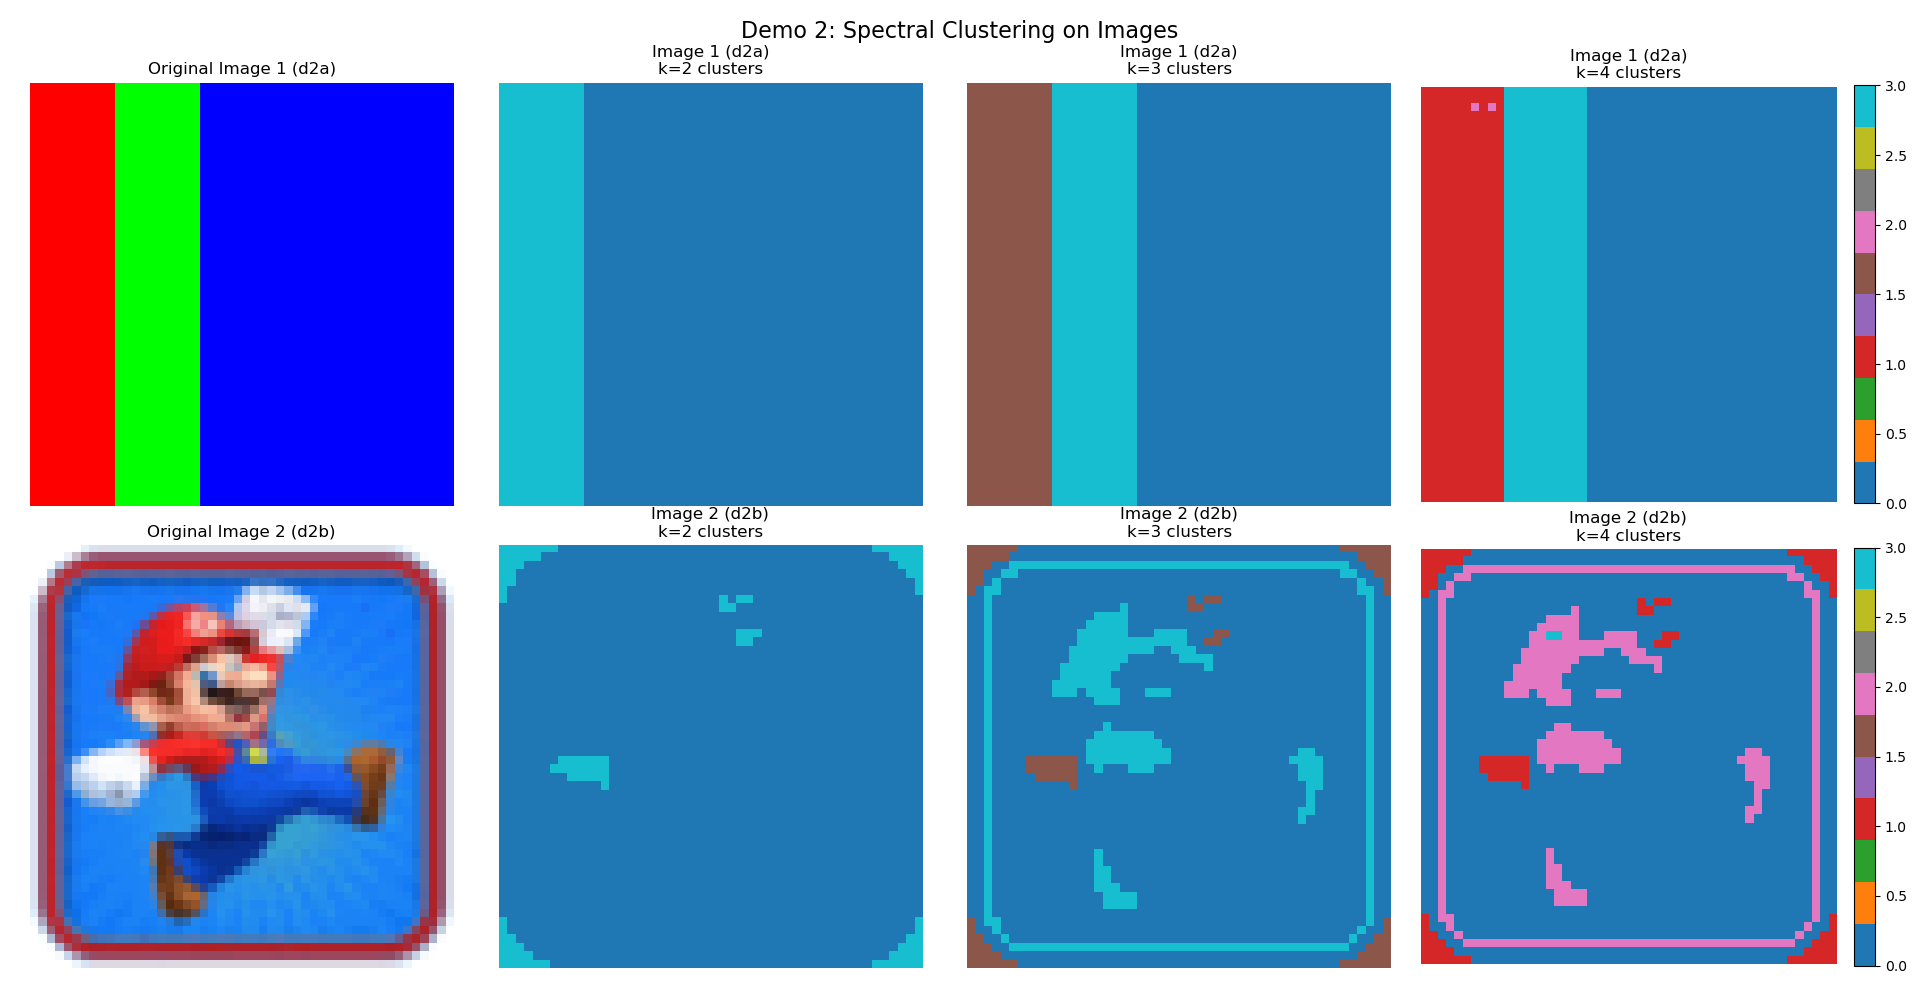
\includegraphics[width=\linewidth]{Figure_2.png}
    \caption{Αποτελέσματα spectral clustering σε εικόνες}\label{figure2}
\end{figure}

\section{Συνάρτηση n\_cuts()}
Η συνάρτηση n\_cuts() βρίσκεται στο αρχείο n\_cuts.py. Η είσοδος της συνάρτησης 
είναι ένα affinity matrix και ο αριθμός των clusters που θα δημιουργηθούν $k$.
Όμοια με τη συνάρτηση spectral\_clustering() κατασκευάζεται το degree matrix 
και υπολογίζεται ο Λαπλασιανός πίνακας $L$. Εδώ η n\_cuts() διαφοροποιείται από τη
spectral\_clustering(), λύνεται η γενικευμένη εξίσωση ιδιοτιμών:

\begin{gather}
    Lx = \lambda Dx \Rightarrow \\
    D^{-1} Lx = \lambda x
\end{gather}
Βρίσκονται ιδιοτιμές και τα αντίστοιχα ιδιοδιανύσματα. Η συνάρτηση 
scipy.sparse.linalg.eigs() καλείται με ορίσμα\-τα k=$k$ και 
which='SM', έτσι ώστε η συνάρτηση να επιστρέψει τις $k$ μικρότερες σε μέτρο
ιδιοτιμές. Τέλος δημιουργεί\-ται ο πίνακας $U$
που έχει στήλες τα ιδιοδιανύσματα του Λαπλασιανού πίνακα $L$ και ομαδοποιούνται
οι γραμμές του $U$ με τη μέθοδο k-means. Έξοδος της συνάρτησης είναι το array 
cluster\_idx που περιέχει τις ετικέτες που δηλώνουν σε ποιό cluster ανήκει κάθε
κόμβος του γράφου.

\section{Συνάρτηση n\_cuts\_recursive()}
Η συνάρτηση βρίσκεται στο αρχείο n\_cuts.py. Οι είσοδοί της είναι ένα affinity matrix 
και τα threshold T1 και T2. Σε κάθε επανάληψη της αναδρομής,
ελέγχεται αν ο αριθμός των pixels που ανήκουν στην τωρινή ετικέτα είναι μικρότερος
από το threshold T1. Αν είναι μικρότερος, η συνάρτηση επιστρέφει 
και η αναδρομή τελειώνει. Αν είναι μεγαλύτερος, βρίσκεται ο υπογράφος με 
όλα τα pixel που ανήκουν στην τωρινή ετικέτα. Ο
υπογράφος αυτός χωρίζεται στα δύο καλώντας τη συνάρτηση n\_cuts() για $k=2$. 
Υπολογίζεται η τιμή n\_cut με κλήση της συνάρτησης calculate\_n\_cut\_va\-lue()
με ορίσματα τις δύο νέες ετικέτες και το affinity matrix του υπογράφου.
Αν η n\_cut είναι μεγαλύτερη από το threshold T2 η συνάρτηση επιστρέφει και τελειώνει η
αναδρομή χωρίς να ληφθεί υπόψιν ο τελευταίος χωρισμός του υπογράφου. Αλλιώς,
καλείται ξανά η n\_cuts\_recursive() για κάθε ένα από τα δύο subclusters 
που δημιουργήθηκαν και η αναδρομή συνεχίζει. Πριν τελειώσει η 
κάθε αναδρομή, η τωρινή ετικέτα αναθέτεται σε όλα τα pixel
του cluster\_idx που ανήκουν  στο τωρινό cluster. Η έξοδος της
συνάρτησης είναι το τελικό cluster\_idx.

\section{Συνάρτηση calculate\_n\_cut\_value()}
Η συνάρτηση αυτή βρίσκεται στο αρχείο n\_cuts.py. Οι είσοδοί της είναι ένα 
affinity matrix που περιγράφει ένα γράφο / μια εικόνα και το cluster\_idx array 
που δηλώνει ποιά pixel της εικόνας ανήκουν σε ποιό cluster. Αναγκαστικά το
cluster\_idx μπορεί να έχει μόνο δύο clusters. Για να σιγουρευτεί η
αλήθεια αυτής της προϋπόθεσης γίνεται έλεγχος. Υπολογίζονται οι 
μετρικές assoc(A,A), assoc(A,V), assoc(B,B) και assoc(B,V), όπου A,B τα δύο
clusters και V ολόκληρος ο γράφος, ο οποίος περιγράφεται από το affinity
matrix της εισόδου και μπορεί να είναι μικρότερος από την αρχική εικόνα. 
Η μετρική assoc() υπολογίζεται ως εξής:

\begin{equation}
    assoc(A,V) = \sum_{i, j} W(i, j)
\end{equation}
όπου $i$ τα indices των κόμβων του affinity πίνακα που ανήκουν στο cluster A
και $j$ τα indices όλων των κόμβων του affinity matrix. Έπειτα υπολογίζεται η 
τιμή n\_cut:

\begin{equation}
    n\_cut = 2 - \left(\frac{assoc(A,A)}{assoc(A,V)} + \frac{assoc(B,B)}{assoc(B,V)}\right)
\end{equation}
η οποία είναι και η έξοδος της συνάρτησης.

\section{Εφαρμογές}
\subsection{demo3a} 
Στο αρχείο demo3a.py γίνεται η επίδειξη της συνάρτησης n\_cuts(). Οι
δοσμένες εικόνες d2a και d2b φορτώνονται από το αρχείο 
dip\_hw\_3.mat. Γίνονται έλεγχοι αν οι εικόνες εισόδου πληρούν τις προϋποθέσεις 
της img\_to\_graph(), δηλαδή να είναι έγχρωμες και οι τιμές τους να κυμαίνονται 
στο διάστημα $[0,1]$. Για κάθε μία από τις δύο εικόνες υπολογίζεται πρώτα το
affinity matrix με τη χρήση της img\_to\_graph(). Για κάθε affinity matrix και 
για τις τιμές $k=2,3,4$ καλείται η συνάρτηση n\_cuts() (συνολικά 6 φορές). Για την
οπτικοποίηση, κάθε cluster από pixels της αρχικής εικόνας έχει διαφορετικό χρώμα
(\autoref{figure3}). Βλέπουμε στην πάνω εικόνα με τις στήλες χρώματος
τα ίδια αποτελέσματα με τη μέθοδο spectral clustering για τιμές $k=2,3$, τα όρια 
των clusters είναι τα όρια των στηλών χρώματος. Για $k=4$ έχουμε περισσότερα
pixels που ανήκουν στο τέταρτο cluster, το οποίο δν προσφέρει καμία πληροφορία σε σχέση με τη μέθοδο 
spectral\_clustering().
Στην κάτω εικόνα βλέπουμε για $k=2$ ότι η σιλουέτα του Mario διαγράφεται 
καλύτερα σε σχέση με τη μέθοδο spectral clustering. Στο ένα cluster ανήκουν 
όλα τα pixel που δεν είναι μπλε και στο
άλλο ανήκουν το background, το παντελόνι και τα μπλε μάτια του Mario. Για $k=3$,
τα clusters χωρίζονται σε κόκκινο-καφέ, άσπρο-χρώμα δέρματος και μπλε. Ακόμα και
αν δεν είχαμε την αρχική εικόνα, θα μπορούσαμε από αυτήν την εικόνα να αναγνωρίσουμε
ότι απεικονίζεται ο Mario. Για $k=4$ η μέθοδος normalized cuts κατάφερε να διαχωρίσει
το σκούρο μπλε του παντελονιού του Mario και το φωτεινό μπλε background σε 
διαφορετικά clusters. Από την άλλη ίσως έχουμε υπερβολική λεπτομέρεια στα σημεία όπου 
τα κόκκινα borders γίνονται μπλε background η οποία δεν είναι ιδιαίτερα βοηθητική.
Ως συμπέρασμα μπορούμε να πούμε ότι η μέθοδος normalized cuts κάνει καλύτερο 
διαχωρισμό σε περίπλοκες φιγούρες και σχήματα από τη μέθοδο spectral clustering, 
ενώ σε απλά σχήματα δεν υπάρχει καμιά σηματνική διαφορά.

\begin{figure}
    \centering
    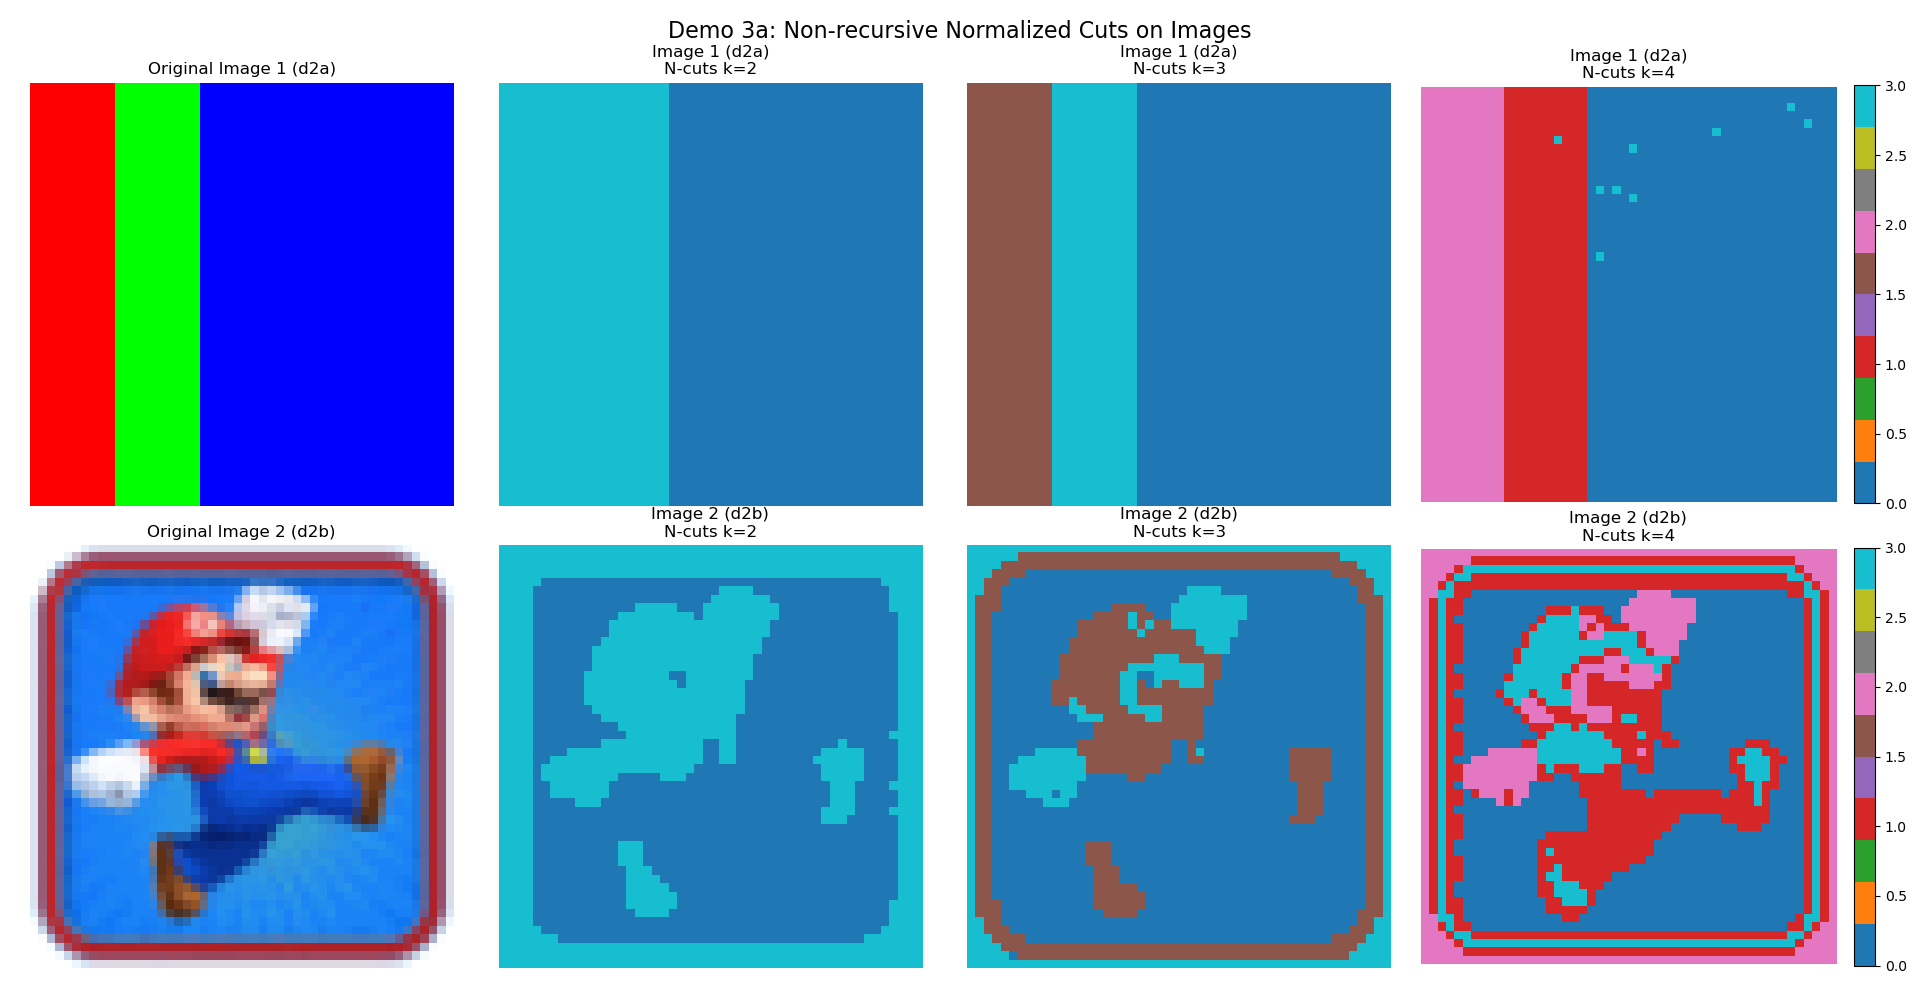
\includegraphics[width=\linewidth]{Figure_3.png}
    \caption{Αποτελέσματα μεθόδου normalized cuts (non-recursive) σε εικόνες}\label{figure3}
\end{figure}

\subsection{demo3b}
Στο αρχείο demo3b.py γίνεται η επίδειξη της μεθόδου recursive normalized cuts. Όμοια
με το demo3a.py φορτώνονται οι δοσμένες εικόνες d2a, d2b και υπολογίζονται τα affinity 
matrices τους με την img\_to\_graph(). Έπειτα εκτελείται το πρώτο βήμα της recursive
n-cuts μεθόδου. Καλείται η συνάρτηση n\_cuts() με ορίσμα\-τα τους πίνακες affinity 
των εικόνων και $k=2$. Υπολογίζεται η τιμή n\_cut καλώντας την συνάρτηση 
calculate\_n\_cut\_value(). Τα ορίσμα\-τά της είναι ο πίνακας affinity και το
array cluster\_idx έξοδος της n\_cuts(). Έπειτα προβάλλεται στην οθόνη η 
αρχική εικόνα, η εικόνα με τα δύο διαφορετικά clusters και η τιμή n\_cut.
Βλέπουμε στην~\autoref{figure4} ότι για $k=2$, τα αποτελέσματα είναι τα 
ίδια με την῀\autoref{figure3}. Η τιμή n\_cut για την πάνω περίπτωση είναι περίπου 0.51 και για 
την κάτω περίπου 0.78. 

\begin{figure}
    \centering
    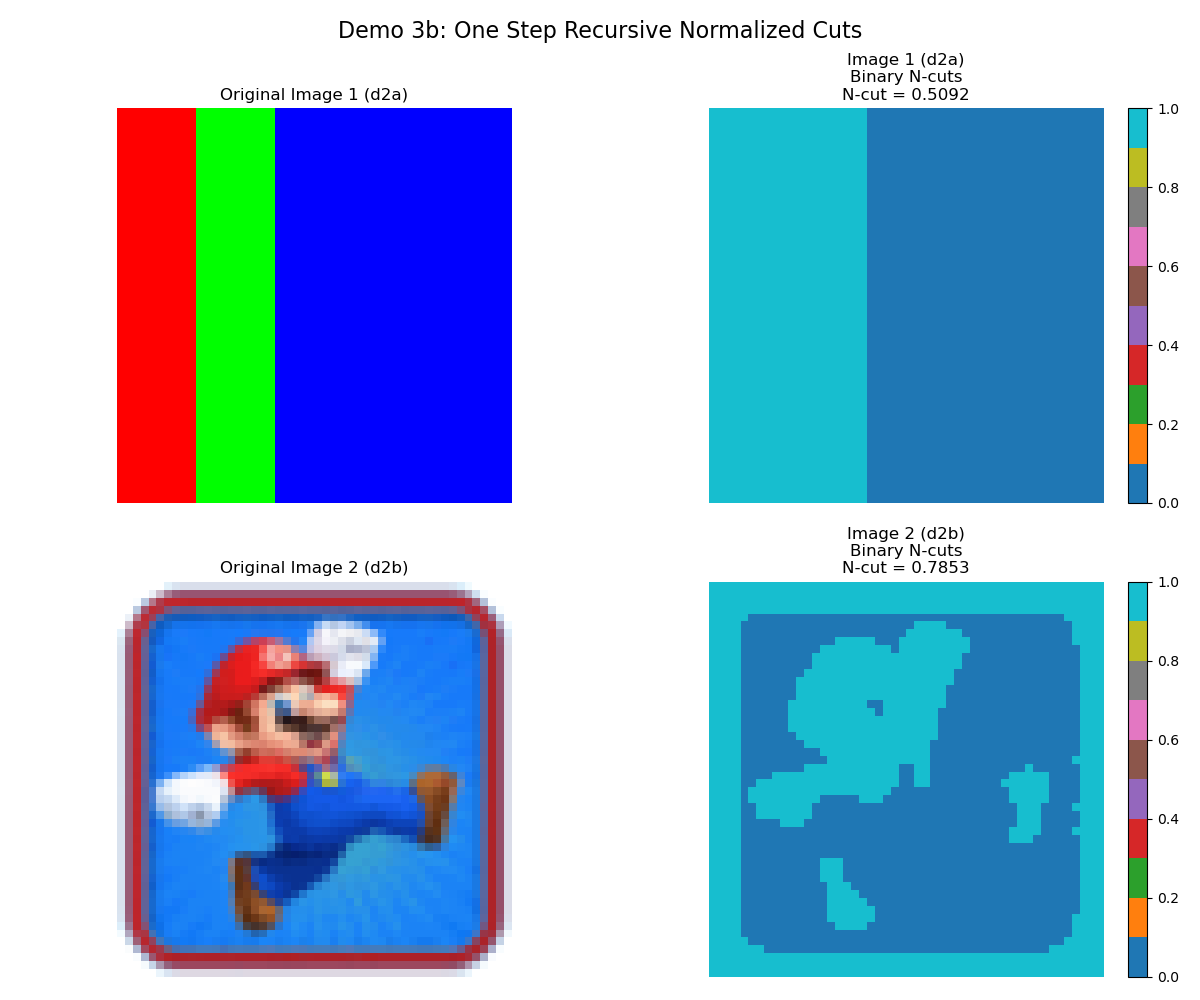
\includegraphics[width=\linewidth]{Figure_4.png}
    \caption{Αποτελέσματα recursive n-cuts μεθόδου για μία επανάληψη}\label{figure4}
\end{figure}

\subsection{demo3c}
Στο αρχείο demo3c.py γίνεται η επίδειξη της ολοκληρωμένης μεθόδου recursive 
normalized cuts. Όμοια με το demo3a.py φορτώνονται οι δοσμένες εικόνες d2a, d2b και υπολογίζονται τα affinity 
matrices τους με την img\_to\_graph(). Έπειτα καλείται η  n\_cuts\_recursive() 
με ορίσματα τον affinity πίνακα του γράφου της εικόνας και thresholds $T1=5$, $T2=0.2$. Βλέπουμε
από την~\autoref{figure5} ότι η αναδρομική μέθοδος δεν έτρεξε ούτε μια φορά και όλα τα pixels
και στις δύο εικόνες είναι σε ένα cluster, το αρχικό. Αυτό είναι το αναμενόμενο
αποτέλεσμα, αφού υπολογίσαμε στο demo3b.py τις n\_cut τιμές των αρχικών εικόνων 
0.51 και 0.78, πολύ μεγαλύτερες από το threshold $T2=0.2$.

Επειδή δεν έχουμε δει ακόμα την n\_cuts\_recursive() με αναδρομία, ξαναέτρεξα το
demo3c.py για $T2=0.8$. Βλέπουμε τα αποτελέσματα στην~\autoref{figure6}. Στην 
πάνω περίπτωση τα αποτελέσματα είναι ακριβώς ίδια για την περίπτωση της 
μη αναδρομικής n-cuts μεθόδου για $k=3$. Για την κάτω περίπτωση είναι 
γενικά παρόμοιο με τη μη-αναδρομική μέθοδο για $k=3$, 
ένα cluster για άσπρο χρώμα και χρώμα δέρματος, ένα cluster 
για καφέ και κόκκινο και ένα cluster για το μπλε. Μπορούμε να
δούμε μικρές διαφορές στα κόκκινα borders, στο ένα γάντι του Mario
και γύρω απο τα χρυσά κουμπιά στη σαλοπέτα του. Προφανώς η σωστή 
λειτουργία της n\_cuts\_recursive() εξαρτάται από την επιλογή 
του threshold $T2$. Μπορούμε να συμπεράνουμε ότι η αναδρομική 
μέθοδος n-cuts με τη μη αναδρομική δεν έχουν μεγάλες διαφορές 
στο αποτέλεσμα. Στην μη αναδρομική μέθοδο η ποιότητα του segmentation
εξαρτάται από τη σωστή επιλογή του $k$ την οποία πρέπει να τη 
διαπιστώσει άνθρωπος πειραματικά, πιθανώς για κάθε εικόνα. Αυτό είναι
μη πρακτικό αν θέλουμε image segmentation χωρίς ανθρώπινη επιτήρηση. 
Ενώ η αναδρομική μέθοδος, εφόσον επιλεχθούν τα κατάλληλα thresholds, 
μπορεί να λαμβάνει η ίδια αποφάσεις για το πότε θα κάνει 
διαχωρισμό και πότε όχι, άρα έχει τη δυνατότητα να δουλέψει και
χωρίς ανθρώπινη επιτήρηση.

\begin{figure}
    \centering
    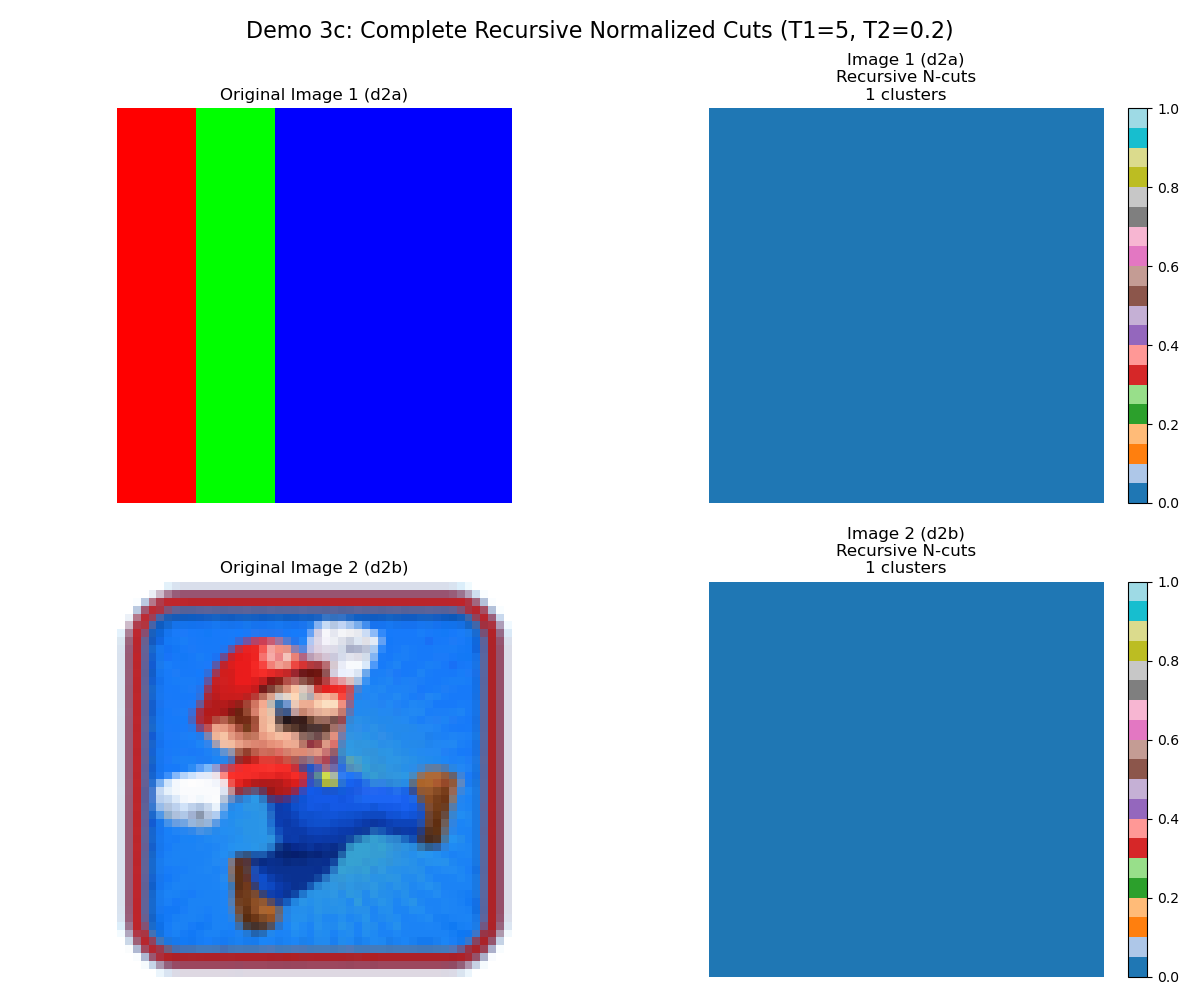
\includegraphics[width=\linewidth]{Figure_5.png}
    \caption{Αποτελέσματα αναδρομικής n-cuts μεθόδου για $T2=0.2$}\label{figure5}
\end{figure}


\begin{figure}
    \centering
    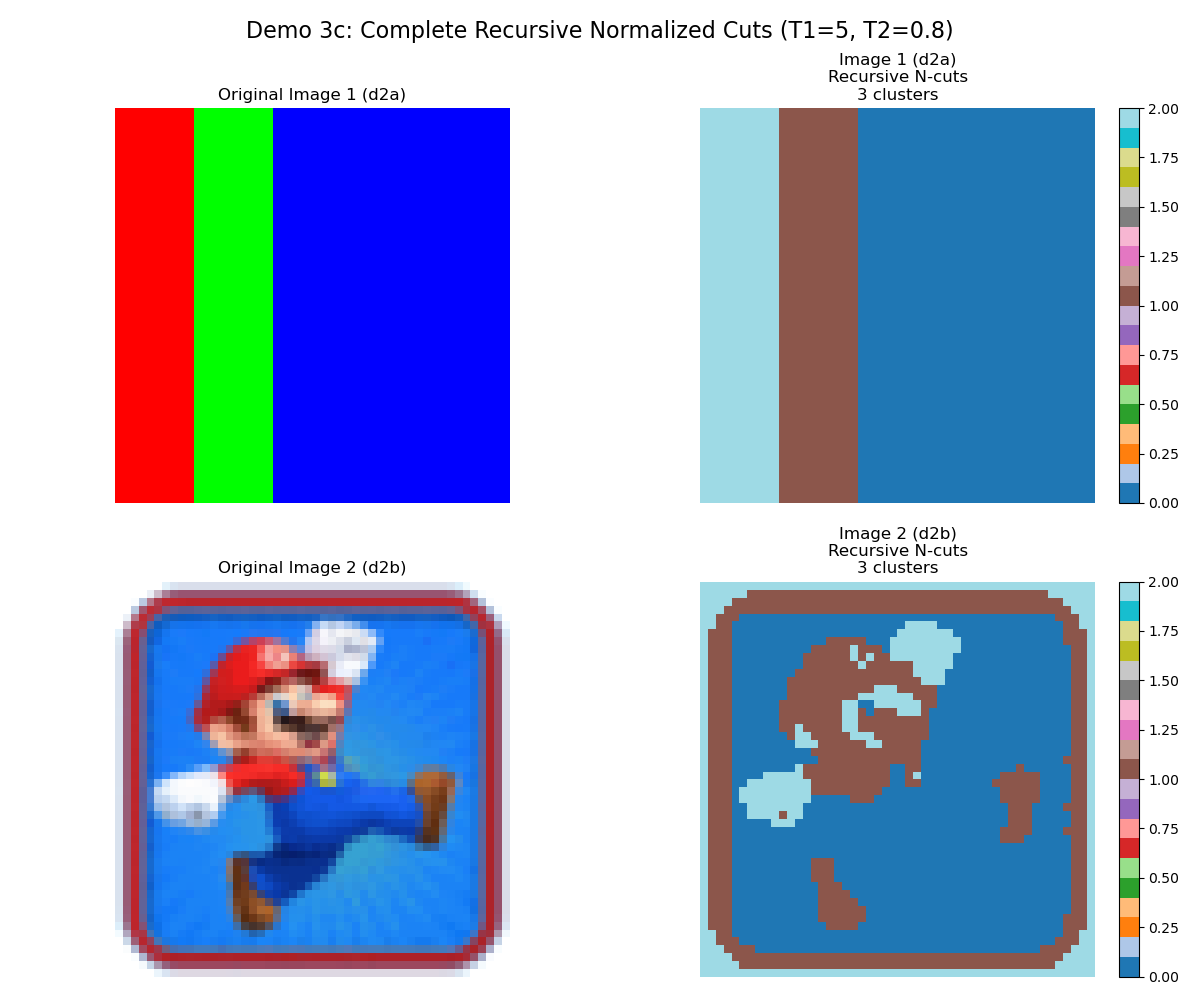
\includegraphics[width=\linewidth]{Figure_6.png}
    \caption{Αποτελέσματα αναδρομικής n-cuts μεθόδου για $T2=0.8$}\label{figure6}
\end{figure}

\end{document}
